\documentclass[Ligatures=TeX,table,brazil,svgnames,usetotalslideindicator,compress,10pt]{beamer}

\usetheme[titleformat=allsmallcaps]{metropolis}

\usepackage{polyglossia}
\setdefaultlanguage{brazil}
\disablehyphenation

\usepackage{minted}

\usetikzlibrary{arrows,positioning,calc}

\usepackage{graphicx}
\graphicspath{{./figuras/}}
\usepackage{subcaption}
\usepackage{xmpmulti}

% \usepackage{textpos}

% \usepackage{mdwlist}
% \usepackage{siunitx}
\usepackage{alltt}
% \usepackage{multicol}
\usepackage{xspace}
\usepackage{multirow}
\usepackage{amsmath}

\usepackage{cancel}

\newcommand{\setcoverbg}{
  \setbeamertemplate{background}
  {\includegraphics[width=\paperwidth,height=\paperheight]{backgrounds/coverbg}}
}
\newcommand{\setintersectionbg}{
  \setbeamertemplate{background}
  {\includegraphics[width=\paperwidth,height=\paperheight]{backgrounds/blank}}
}
\newcommand{\setsectionbg}{
  \setbeamertemplate{background}
  {\includegraphics[width=\paperwidth,height=\paperheight]{backgrounds/slidebg2}}
}

\setbeamertemplate{caption}{default}

\title{MCTA025-13 - Sistemas Distribuídos}
\subtitle{Nomes}

\author{Emilio Francesquini}
\institute{Centro de Matemática, Computação e Cognição\\ Universidade Federal do ABC}
\date{18 de julho de 2018}

\begin{document}

\setcoverbg
\maketitle

\setsectionbg

\begin{frame}
  \frametitle{Disclaimer}
  \begin{itemize}
  \item Estes slides foram preparados para o curso de \textbf{Sistemas
      Distribuídos na UFABC}.
  \item Este material pode ser usado livremente desde que sejam
    mantidos, além deste aviso, os créditos aos autores e
    instituições.
  \item Estes slides foram adaptados daqueles originalmente preparados
    (e gentilmente cedidos) pelo professor \textbf{Daniel Cordeiro, da
      EACH-USP} que por sua vez foram baseados naqueles
    disponibilizados online pelos autores do livro ``Distributed
    Systems'', 3ª Edição em:
    \url{https://www.distributed-systems.net}.
  \end{itemize}
\end{frame}

\begin{frame}
  \frametitle{Nomeação de entidades}
  \begin{itemize}
  \item Nomes, identificadores e endereços
  \item Resolução de nomes
  \item Implementação de um espaço de nomes
  \end{itemize}
\end{frame}

\begin{frame}
  \frametitle{Nomes}
  \begin{block}{Essencialmente}
    Nomes são usados para denotar entidades em um sistema
    distribuído. Para realizar operações em uma entidade, é preciso
    ter acesso a ela usando um \alert{ponto de acesso}. Pontos de
    acessos são entidades que são identificadas por um
    \alert{endereço}.
  \end{block}

\end{frame}

\begin{frame}
  \frametitle{Identificadores}
  \begin{block}{Nomes ``puros''}
    são nomes que não tem significado próprio; são apenas strings
    aleatórias. Nomes puros podem ser usados apenas para comparação.
  \end{block}

  \begin{block}{Identificador}
    Um nome que possui as seguintes propriedades:
    \begin{enumerate}
    \item Cada identificador se refere a, no máximo, uma entidade
    \item Cada entidade é referenciada por, no máximo, um identificador
    \item Um identificador sempre se refere à mesma entidade (reutilização de identificadores é proibida)
    \end{enumerate}
  \end{block}
\end{frame}

\section{Espaço de nomes plano}

\begin{frame}
  \frametitle{Espaço de nomes plano}
  \begin{alertblock}{Problema}
    Dado um nome \alert{não estruturado} (ex: um identificador), como localizar seu \alert{ponto de acesso}?
    \begin{itemize}
    \item Solução simples (broadcasting)
    \item Abordagens baseadas em um local pré-determinado (\textit{home-based})
    \item Tabelas de hash distribuídas (P2P estruturado)
    \item Serviço hierárquico de nomes
    \end{itemize}
  \end{alertblock}
\end{frame}

\begin{frame}
  \frametitle{Soluções simples}
  \begin{block}{Broadcasting}
    Solução: fazer o \textit{broadcast} do ID, requisitando que a entidade devolva seu endereço
    \begin{itemize}
    \item Não escala para além de redes locais
    \item Requer que todos os processos escutem e processem os pedidos de localização
    \end{itemize}

    \begin{block}{Address Resolution Protocol (ARP)}
      Para encontrar o endereço MAC associado a um endereço IP, faz o \textit{broadcast} da consulta ``quem tem esse endereço IP?''
    \end{block}
  \end{block}
\end{frame}

\begin{frame}
  \frametitle{Soluções simples}

  \begin{block}{Ponteiros de redirecionamento}
    Solução: quando uma entidade se mover, ela deixa para trás um ponteiro para sua nova localização
    \begin{itemize}
    \item Dereferenciamento pode ser automático e invisível para o cliente, basta seguir a sequência de ponteiros
    \item Atualize a referência do ponteiro quando o local atual for encontrado
    \item Problemas de escalabilidade geográfica (que podem requerer um mecanismo separado para redução da sequência)
      \begin{itemize}
      \item Sequencias longas não são tolerantes à falhas
      \item Maior latência de rede devido ao processo de dereferenciamento
      \end{itemize}
    \end{itemize}
  \end{block}
\end{frame}

\begin{frame}
  \frametitle{Abordagens baseadas em local pré-determinado}
  Faça com que um local fixo (sua ``casa'') sempre saiba onde a entidade está:
  \begin{itemize}
  \item O endereço pré-determinado é registrado em um serviço de nomes
  \item O endereço mantém um registro do \alert{endereço externo} da entidade
  \item O cliente primeiro contacta o endereço pré-determinado e depois continua para seu endereço externo
  \end{itemize}
\end{frame}

\begin{frame}
  \frametitle{Abordagens baseadas em local pré-determinado}

  Princípio do endereçamento IP móvel:

  \begin{figure}
    \centering
  \includegraphics[width=0.8\textwidth]{05-03}
  \end{figure}
\end{frame}

\begin{frame}
  \frametitle{Abordagens baseadas em local pré-determinado}

  \begin{block}{Abordagem em dois níveis}
    Mantenha um registro das entidades que foram ``visitadas'':
    \begin{itemize}
    \item Verifique o endereço local primeiro
    \item Se falhar, só então vá para o endereço pré-determinado
    \end{itemize}

    \begin{block}{Problemas}
      \begin{itemize}
      \item O endereço pré-determinado deve existir enquanto a entidade existir
      \item O endereço é \alert{fixo} e pode se tornar desnecessário se a entidade se mover permanentemente
      \item Escalabilidade geográfica ruim (a entidade pode estar do lado do cliente)
      \end{itemize}
    \end{block}
  \end{block}

  \textbf{Pergunta:} como resolver o problema da mudança permanente?
  (talvez com outro nível de endereçamento (DNS))

\end{frame}

\begin{frame}
  \frametitle{Tabelas de hash distribuídas (DHT)}
  \begin{block}{Chord}
    Considere que os nós estejam organizados em forma de \alert{anel lógico}
    \begin{itemize}
    \item A cada nó é atribuído um identificador aleatório de $m$-bits
    \item A cada entidade é atribuído uma única \alert{chave} de $m$-bits
    \item Entidades com chave $k$ estão sob a jurisdição do nó com o menor $id \ge k$ (seu sucessor)
    \end{itemize}
  \end{block}

  \begin{exampleblock}{Solução ruim}
    Faça com que cada nó mantenha o registro de seus vizinhos e faça uma busca linear ao longo do anel
  \end{exampleblock}

  \begin{block}{Notação}
    Chamamos de nó $p$ o nó cujo identificador é $p$.
  \end{block}

\end{frame}

\begin{frame}
  \frametitle{DHTs: finger tables}

  Ideia:
  \begin{itemize}
  \item cada no $p$ mantém um \alert{finger table} $FT_p[]$ com no máximo $m$ entradas
    \[ FT_p[i] = succ(p+2^{i-1}) \]
    $FT_p[i]$ aponta para o primeiro nó que sucede $p$ com distância de pelo menos $2^{i-1}$ posições
  \item Para procurar por uma chave $k$, o nó $p$ encaminha o pedido para o nó com índice $j$ tal que:
    \[ q = FT_p[j] \leq k < FT_p[j+1]  \]
  \item Se $p < k < FT_p[1]$, a requisição é encaminhada para $FT_p[1]$
  \end{itemize}

\end{frame}

\begin{frame}
  \frametitle{DHTs: finger tables}
  \begin{figure}
    \centering
    \includegraphics[width=0.75\textwidth]{05-04}
  \end{figure}
\end{frame}

\begin{frame}[fragile]
  \frametitle{Chord em Python}
\scriptsize
\begin{minted}{python}
class ChordNode:
  def finger(self, i):
    succ = (self.nodeID + pow(2, i-1)) % self.MAXPROC    # succ(p+2^(i-1))
    lwbi = self.nodeSet.index(self.nodeID)               # self in nodeset
    upbi = (lwbi + 1) % len(self.nodeSet)                # next neighbor
    for k in range(len(self.nodeSet)):                   # process segments
      if self.inbetween(succ, self.nodeSet[lwbi]+1, self.nodeSet[upbi]+1):
        return self.nodeSet[upbi]                        # found successor
      (lwbi,upbi) = (upbi, (upbi+1) % len(self.nodeSet)) # next segment

  def recomputeFingerTable(self):
    self.FT[0]  = self.nodeSet[self.nodeSet.index(self.nodeID)-1] # Pred.
    self.FT[1:] = [self.finger(i) for i in range(1,self.nBits+1)] # Succ.

  def localSuccNode(self, key):
    if self.inbetween(key, self.FT[0]+1, self.nodeID+1): # in (FT[0],self]
      return self.nodeID                                 # responsible node
    elif self.inbetween(key, self.nodeID+1, self.FT[1]): # in (self,FT[1]]
      return self.FT[1]                                  # succ. responsible
    for i in range(1, self.nBits+1):                     # rest of FT
      if self.inbetween(key, self.FT[i], self.FT[(i+1) % self.nBits]):
        return self.FT[i]                                # in [FT[i],FT[i+1])
\end{minted}
\end{frame}

\begin{frame}
  \frametitle{Exploração de proximidade da rede}
  \begin{block}{Problema:}
A organização lógica dos nós em uma rede de overlay pode levar à transferência de mensagens de forma errática na Internet: os nós $k$ e $succ(k+1)$ podem estar muito longes um do outro.
\end{block}

\begin{block}{Soluções}
\begin{itemize}
    \item<2-> \alert{Atribuição ciente da rede:} ao atribuir um ID ao nó, assegure-se de que nós próximos no espaço de endereçamento estão próximos na rede real. \textbf{Pode ser muito complicado.}
    \item<3-> \alert{Roteamento de proximidade:} mantenha mais de um sucessor possível e encaminhe a mensagem para o mais próximo. Ex: no Chord, $FT_p[i]$ aponta para o primeiro nó em $INT = [p+2^{i-1},p+2^i-1]$. O nó $p$ pode guardar também ponteiros para outros nós em $INT$.
    \item<4-> \alert{Seleção de vizinho por proximidade:} quando houver uma escolha para determinar quem será seu vizinho, escolha o mais próximo.
    \end{itemize}
  \end{block}
\end{frame}

\begin{frame}
  \frametitle{Serviços de localização hierárquicos (HLS)}

  Ideia:
  \begin{block}{}
    Construir uma árvore de busca em larga escala onde a rede é dividida em domínios hierárquicos. Cada domínio é representado por um diretório de nós separado.
  \end{block}

  \begin{figure}
    \centering
    \includegraphics[width=0.8\textwidth]{05-05}
  \end{figure}

\end{frame}

\begin{frame}
  \frametitle{HLS: organização em árvores}
  \begin{block}{Invariantes}
    \begin{itemize}
    \item Endereço da entidade $E$ é armazenado numa folha ou nó intermediário
    \item Nós intermediários contém um ponteiro para um filho \textit{sse} a subárvore cuja raiz é o filho contenha o endereço da entidade
    \item A raiz conhece todas as entidades
    \end{itemize}
  \end{block}

  \begin{figure}
    \centering
    \includegraphics[width=0.8\textwidth]{05-06}
  \end{figure}
\end{frame}

\begin{frame}
  \frametitle{HLS: consulta}
  Princípios básicos:
  \begin{itemize}
  \item Comece a busca pelo nó folha local
  \item Se o nó souber sobre $E$, seguir o ponteiro pra baixo, senão continue a subir
  \item Continue subindo até encontrar a raiz
  \end{itemize}

  \begin{figure}
    \centering
    \includegraphics[width=0.8\textwidth]{05-07}
  \end{figure}
\end{frame}

\begin{frame}
  \frametitle{HLS: inserção}

  \begin{tabular}{cc}
    \includegraphics[scale=0.8]{05-08a} & \includegraphics[scale=0.8]{05-08b}
  \end{tabular}

  \begin{block}{}
    \begin{enumerate}
    \item[(a)] um pedido de inserção é encaminhado ao primeiro nó que conhece a entidade E
    \item[(b)] uma cadeia de ponteiros de redirecionamento é criada até o nó folha
    \end{enumerate}
  \end{block}

\end{frame}

% \begin{frame}
%   \frametitle{O HLS é escalável?}
%   \begin{block}{Observação}
%     Um problema no projeto parece fazer o nó raiz manter um registro de \alert{todos} os identificadores $\Rightarrow$ fazer uma distinção entre o \alert{projeto lógico} e a \alert{implementação física}
%   \end{block}

%   \begin{block}{Notação}
%     \begin{itemize}
%     \item Assuma que há um total de $N$ computadores físicos $\{H_1, H_2, \dots, H_N\}$. Cada computador é capaz de executar um ou mais servidores de localização.
%     \item $D_K(A)$ denota o domínio no nível $k$ que contém o endereço $A$; $k=0$ denota o domínio raiz
%     \item $LS_k(E,A)$ denota o único servidor de localização em $D_k(A)$ responsável por
%     \end{itemize}
%   \end{block}

% \end{frame}

\section{Espaços de nomes estruturados}

\begin{frame}
  \frametitle{Espaço de nomes}
  \begin{block}{Ideia}
    Um grafo no qual um \alert{nó folha} representa uma entidade que tem um nome. Um \alert{diretório de nós} é uma entidade que se refere a outros nós.
  \end{block}

  \begin{figure}
    \centering
    \includegraphics[width=0.8\textwidth]{05-09}
  \end{figure}

  \begin{block}{Nota:}
    Um diretório contém uma tabela de pares \emph{(identificador do nó, rótulo da aresta)}
  \end{block}
\end{frame}

\begin{frame}
  \frametitle{Espaço de nomes estruturado}
  \begin{block}{Observação}
    É fácil guardar em um nó vários tipos de atributos para descrever propriedades da entidade que o nó representa:
    \begin{itemize}
    \item tipo da entidade
    \item identificador da entidade
    \item endereço da localização da entidade
    \item \textit{nicknames}
    \item ...
    \end{itemize}
  \end{block}

  \pause
  \begin{alertblock}{Nota:}
    Nós de diretórios também podem ter atributos, além de guardar a tabela com os pares (identificador, rótulo)
  \end{alertblock}

\end{frame}

\begin{frame}
  \frametitle{Resolução de nomes}
  \begin{alertblock}{Problema:}
    Para resolver um nome precisamos de um diretório. Como encontrar esse nó inicialmente?
  \end{alertblock}

  \begin{block}{Mecanismo de closure}
    \begin{itemize}
      \item \texttt{cmcc.ufabc.edu.br}: inicia em um servidor DNS
  \item \texttt{/home/e.francesquini/Maildir}: inicia em um servidor de arquivos NFS local (busca potencialmente recursiva)
  \item \texttt{00551149968327}: disca um número de telefone
  \item \texttt{200.133.215.63}: rota para um servidor da UFABC
    \end{itemize}
  \end{block}

\end{frame}

\begin{frame}
  \frametitle{Links para nomes}
  \begin{block}{Hard link}
    O que descrevemos até agora foi um \alert{caminho}: um nome que é resolvido ao seguir um caminho específico em um grafo de nomes, indo de um nó para outro.
  \end{block}
\end{frame}

\begin{frame}
  \frametitle{Links para nomes}
  \begin{block}{Soft link}
    Permite que um nó $O$ mantenha o \alert{nome} de outro nó:
    \begin{itemize}
    \item Primeiro resolva o nome de $O$ (o que leva ao nó $O$)
    \item Leia o conteúdo de $O$, que leva ao \texttt{nome}
    \item A resolução do nome continua com \texttt{nome}
    \end{itemize}
  \end{block}
\end{frame}

\begin{frame}
  \frametitle{Links para nomes}
  \begin{figure}
    \centering
    \includegraphics[width=\textwidth]{05-11}
  \end{figure}

  \begin{alertblock}{Observação:}
    O nó \texttt{n5} tem apenas um nome.
  \end{alertblock}

\end{frame}

\begin{frame}
  \frametitle{Mounting/Mapping}
  Permite fazermos uma \alert{junção} (\emph{merge}) dois espaços de nomes distintos
  \begin{itemize}
  \item Múltiplos discos/sistemas de arquivo na mesma máquina
  \item Múltiplos computadores na mesma rede
  \end{itemize}
  \begin{figure}
    \centering
    \includegraphics[width=0.8\textwidth]{05-14}
  \end{figure}

\end{frame}

\begin{frame}
  \frametitle{Plan9 - O Filme}

  \begin{figure}
    \centering
    \begin{minipage}{0.45\textwidth}
      \centering
        \includegraphics[width=0.9\textwidth]{plan9.jpg}
    \end{minipage}\hfill
    \begin{minipage}{0.45\textwidth}
        \centering
        \includegraphics[width=0.9\textwidth]{bl.jpg}\\
        \includegraphics[width=0.9\textwidth]{plan9b.jpg}
    \end{minipage}
  \end{figure}

\end{frame}

\begin{frame}
  \frametitle{Plan9 - O Sistema Operacional}
  \begin{figure}
    \centering
    \begin{minipage}{0.3\textwidth}
      \centering
      \includegraphics[width=0.9\textwidth]{planso.jpg}
    \end{minipage}\hfill
    \begin{minipage}{0.65\textwidth}
      \centering
      \begin{itemize}
      \item No \textbf{Plan9} (1995) os recursos de hardware (discos,
        I/O, placas de rede, \ldots) e de software (processos,
        memória, \ldots) são \alert{mapeados para um único sistema de
          nomes}
      \item Usava fortemente o conceito de pontos de montagem
      \item Sua abordagem é usada até hoje, com algumas modificações,
        na maior parte dos sistemas operacionais.
      \end{itemize}
    \end{minipage}
  \end{figure}

\end{frame}


\begin{frame}
  \frametitle{Implementação de espaços de nomes}
  \begin{block}{Problema:}
    Distribuir o processo de resolução de nomes, bem como o
    gerenciamento do espaço de nomes, em várias máquinas, de forma a
    distribuir o grafo de nomes para garantir\textbf{ escalabilidade e
    disponibilidade}.
  \end{block}
\end{frame}

\begin{frame}
  \frametitle{Impl. de espaços de nomes - Distribuição}
  \begin{block}{Três níveis distintos:}
    \begin{enumerate}
    \item \alert{Nível global:} consiste de um diretório de nós de
      alto nível. Suas principais características são que os nós do
      diretório devem ser gerenciados em conjunto por
      \textbf{diferentes administradores} e que há uma relativa
      \textbf{estabilidade nos nomes}, ou seja, as entradas do
      diretório são modificadas muito raramente
    \item \alert{Nível de administração:} nós de diretório de nível
      intermediário. Podem ser agrupagos e \textbf{cada grupo
      pode ser responsabilidade de um administrador diferente}. Apesar de
      estáveis, mudam com mais frequência do que entradas no nível
      global
    \item \alert{Nível gerencial:} nós de nível inferior que
      \textbf{pertencem a um único administrador}. O problema
      principal é mapear os nós de diretório aos servidores de nomes
      local. \textbf{Mudanças regulares} ocorrem neste nível.
    \end{enumerate}
  \end{block}
\end{frame}

\begin{frame}
  \frametitle{Implementação de espaços de nomes}
  \includegraphics[width=\textwidth]{05-13}
\end{frame}

\begin{frame}
  \frametitle{Implementação de espaços de nomes}

  \begin{center}
    \small
    \renewcommand{\arraystretch}{1.1}
    \begin{tabular}{|l|l|l|l|}\hline
      \alert{\textbf{Item}} & \alert{\textbf{Global}} & \alert{\textbf{Administração}} & \alert{\textbf{Gerencial}}\\ \hline
      1 & Mundial	& Organização 	& Departamento 	\\ \hline
      2 & Poucos 		& Muitos 			& Qdes. enormes 	\\ \hline
      3 & Segundos 	& Milissegundos 	& Imediato 	\\ \hline
      4 & Tardio 		& Imediato 	& Imediato 	\\ \hline
      5 & Muitos 		& Nenhum ou poucos 	& Nenhum 			\\ \hline
      6 & Sim 		& Sim 			& Às vezes 	\\ \hline\hline
      \multicolumn{2}{|l|}{1: Escala geográfica} & \multicolumn{2}{l|}{4: Propagação de atualizações} \\
      \multicolumn{2}{|l|}{2: \# Nós} 			& \multicolumn{2}{l|}{5: \# Réplicas} \\
      \multicolumn{2}{|l|}{3: Responsividade} 	& \multicolumn{2}{l|}{6: Cache no lado do cliente?} \\ \hline
    \end{tabular}
  \end{center}

\end{frame}

\begin{frame}
  \frametitle{Resolução de nomes iterativa}


  \begin{enumerate}

  \item \texttt{resolve(dir,[name1,...,nameK])} enviado para \texttt{Server0} responsável por \texttt{dir}
  \item \texttt{Server0} resolve \texttt{resolve(dir,name1)} $\rightarrow$ \texttt{dir1}, devolve a identificação
     (endereço) de \texttt{Server1}, que contém \texttt{dir1}.
  \item Cliente envia \texttt{resolve(dir1,[name2,...,nameK])} para \texttt{Server1}, etc.

  \end{enumerate}

  \begin{figure}
    \centering
    \includegraphics[width=0.8\textwidth]{05-15}
  \end{figure}

\end{frame}

\begin{frame}
  \frametitle{Resolução de nomes recursiva}
  \begin{enumerate}
  \item \texttt{resolve(dir,[name1,...,nameK])} enviado a \texttt{Server0}, responsável por \texttt{dir}
  \item \texttt{Server0} resolve \texttt{resolve(dir,name1)} $\rightarrow$ \texttt{dir1} e envia
    \texttt{resolve(dir1,[name2,...,nameK])} para \texttt{Server1}, que contém \texttt{dir1}.
  \item \texttt{Server0} espera pelo resultado de  \texttt{Server1} e o devolve para o cliente.
  \end{enumerate}

  \begin{figure}
    \centering
    \includegraphics[width=0.8\textwidth]{05-16}
  \end{figure}

\end{frame}

\begin{frame}
  \frametitle{Uso de cache na resolução recursiva}

  \begin{center}
    \sffamily\scriptsize
    \begin{minipage}{18cm}
      \renewcommand{\arraystretch}{1.2}
      \begin{tabular}{@{}|c|c|c|c|c|c|}\hline
        Servidor 		& Deveria 				& Procura por 		& Envia para 		& Recebe e 			& Devolve 				\\
        para o nó 	& resolver 				&  				& filho 			& and faz cache 		& ao solicitante 			\\ \hline
        cs 			& $<$ftp$>$ 			& \#$<$ftp$>$ 	& --- 				& --- 				& \#$<$ftp$>$ 			\\ \hline
        vu 			& $<$cs,ftp$>$ 			& \#$<$cs$>$ 	& $<$ftp$>$ 		& \#$<$ftp$>$ 		& \#$<$cs$>$			\\
 		            &  						&  				&  					&  					& \#$<$cs, ftp$>$ 		\\ \hline
        nl 			& $<$vu,cs,ftp$>$ 		& \#$<$vu$>$ 	& $<$cs,ftp$>$ 		& \#$<$cs$>$ 		& \#$<$vu$>$			\\
 		            &  						&  				&  					& \#$<$cs,ftp$>$ 	& \#$<$vu,cs$>$ 		\\
 		            &  						&  				&  					&  					& \#$<$vu,cs,ftp$>$ 	\\ \hline
        root 		& $<$nl,vu,cs,ftp$>$ 	& \#$<$nl$>$ 	& $<$vu,cs,ftp$>$ 	& \#$<$vu$>$ 		& \#$<$nl$>$			\\
 		            &  						&  				&  					& \#$<$vu,cs$>$ 	& \#$<$nl,vu$>$			\\
 		            &  						&  				&  					& \#$<$vu,cs,ftp$>$ & \#$<$nl,vu,cs$>$		\\
 		            &  						&  				&  					&  					& \#$<$nl,vu,cs,ftp$>$	\\ \hline
      \end{tabular}
    \end{minipage}
  \end{center}

\end{frame}

\begin{frame}
  \frametitle{Problemas de escalabilidade}
  \begin{alertblock}{Escalabilidade de tamanho}
    Devemos garantir que os servidores possam lidar com um grande número de requisições por unidade de tempo. Servidores de alto nível podem estar com problemas sérios.
  \end{alertblock}

  \pause
  \begin{block}{Solução:}
    Assuma (pelo menos nos níveis global e de administração) que os conteúdos dos nós mudam muito pouco. Assim podemos aplicar replicação extensivamente, mapeando nós a múltiplos servidores e começar a resolução de nomes no servidor mais próximo.
  \end{block}

  \pause
  \begin{block}{Observação:}
    Um atributo importante em muitos nós é o seu \alert{endereço} (onde a entidade pode ser localizada). Replicação faz com que servidores de nomes em larga escala sejam inadequados para localizar entidades móveis.
  \end{block}
\end{frame}

\begin{frame}
  \frametitle{Problemas de escalabilidade}
  \begin{alertblock}{Escalabilidade geográfica}
    Precisamos garantir que a resolução de nomes escale mesmo em grandes distâncias geográficas
  \end{alertblock}

  \begin{figure}
    \centering
    \includegraphics[width=0.8\textwidth]{05-18}
  \end{figure}

  \begin{block}{Porém:}
    Ao mapear nós em servidores que podem ser localizados em qualquer lugar, nós acabamos introduzindo uma dependência de localização implícita.
  \end{block}
\end{frame}

\begin{frame}
  \frametitle{Exemplo: DNS decentralizado}
  \begin{block}{Ideia básica}
    Pegue um nome DNS completo, crie um hash com chave $k$ e use um sistema DHT que permita consulta a chaves. \alert{Desvantagem:} você não pode pedir por todos os nós em um subdomínio (mas pouca gente faz isso)
  \end{block}

  \begin{block}{Informação em um nó:}
    \footnotesize
    \renewcommand{\arraystretch}{1.2}
    \begin{center}
      \begin{tabular}{|l|l|l|}\hline
        SOA & Zone & Holds info on the represented zone \\ \hline
        A & Host & IP addr. of host this node represents \\ \hline
        MX & Domain & Mail server to handle mail for this node \\ \hline
        SRV & Domain & Server handling a specific service \\ \hline
        NS & Zone & Name server for the represented zone \\ \hline
        CNAME & Node & Symbolic link  \\ \hline
        PTR & Host & Canonical name of a host \\ \hline
        HINFO & Host & Info on this host \\ \hline
        TXT & Any kind & Any info considered useful \\ \hline
      \end{tabular}
    \end{center}

  \end{block}

\end{frame}

\begin{frame}
  \frametitle{DNS no Pastry}
  \begin{block}{Pastry}
    Sistema baseado em DHT que funciona com \alert{prefixos} de chaves. Considere um sistema onde as chaves pertençam a um espaço de números de 4 dígitos. Um nó com ID 3210 mantém informações sobre os seguintes nós:
  \end{block}
  \begin{center}\footnotesize
      \begin{tabular}{lclc} \\
        $n_k$ & prefix of ID($n_k$) &         $n_k$ & prefix of ID($n_k$) \\ \hline
        $n_0$ & 0  &
        $n_1$ &  1  \\
        $n_2$ &  2  &
        $n_{30}$ &  30  \\
        $n_{31}$ &  31  &
        $n_{33}$ &  33  \\
        $n_{320}$ &  320  &
        $n_{322}$ &  322  \\
        $n_{323}$ &  323 & \\
      \end{tabular}
    \end{center}


  \begin{alertblock}{Notas:}
    O nó 3210 é responsável pelas chaves com prefixo 321. Se ele receber uma requisição pela chave 3012, ela será reencaminhada ao no $n_{30}$. Para DNS: um nó responsável pela chave $k$ armazena os registro DNS de nomes cujo valor do hash seja $k$.
  \end{alertblock}
\end{frame}

\begin{frame}
  \frametitle{Replicação de registros}
  \begin{block}{Definição}
    \alert{Replicação no nível $i$} -- registro é replicado em todos os nós com prefixo $i$. \alert{Nota:} \# saltos para procurar por um registro no  nível $i$ normalmente é $i$.
  \end{block}

  \begin{block}{Observação:}
    Seja $x_i$ a fração dos nomes DNS mais populares que deveriam ser replicados no nível $i$. Então:
     \[x_i = \left [ \frac{d^i ( \log N - C )}{1 + d + \cdots + d^{\log N - 1}} \right ]^{1/(1-\alpha)}\]
     onde $N$ é o número total de nós, $d = b^{(1-\alpha)/\alpha}$ e $\alpha \approx 1$, assumindo que a ``popularidade'' siga a distribuição de Zipf: a frequência do n-ésimo item mais popular é proporcional a $1/n^\alpha$
  \end{block}
\end{frame}

\begin{frame}
  \frametitle{Replicação de registros}
  \begin{block}{}
    Se quisermos que o número médio de consultas para a resolução de um nome DNS seja $C=1$, então com $b=4$, $\alpha=0,9$, $N = 10.000$ e $1.000.000$ registros

    \begin{center}
      \begin{tabular}{r@{\ }l}
        61 & registros mais populares devem ser \\ & replicados no nível 0 \\
        284 & próximos registros mais populares no nível  1 \\
        1323 & próximos registros mais populares no nível 2 \\
        6177 & próximos registros mais populares no nível 3 \\
        28826 & próximos registros mais populares no nível 4 \\
        134505 & próximos registros mais populares no nível 5 \\
        o resto & não deve ser replicado
      \end{tabular}
    \end{center}

  \end{block}
\end{frame}

\section{Nomeação baseada em atributos}

\begin{frame}
  \frametitle{Nomeação baseada em atributos}
  \begin{block}{Observação}
    Em muitos casos, é mais conveniente nomear e procurar entidades pelos seus \alert{atributos} $\Rightarrow$ serviços tradicionais de diretórios (ex: páginas amarelas).
  \end{block}

  \pause
  \begin{alertblock}{Problema:}
    Operações de consulta podem ser muito caras, já que necessitam que os valores dos atributos procurados correspondam aos valores reais das entidades. Em princípio, teríamos que inspecionar todas as entidades.
  \end{alertblock}

  \pause
  \begin{block}{Solução:}
    Implementar serviços de diretórios básicos (tais como bancos de dados) e combiná-los com os sistemas de nomes estruturados tradicionais.
  \end{block}
\end{frame}

\begin{frame}[fragile]
  \frametitle{Exemplo: LDAP}
  \begin{figure}
    \centering
    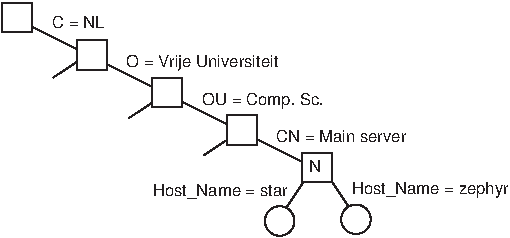
\includegraphics[width=0.6\textwidth]{05-23}
  \end{figure}

  \begin{center}\tiny
    \renewcommand{\arraystretch}{1.5}
    \begin{tabular}{|l|l|c|l|l|} \cline{1-2}\cline{4-5}
      \alert{\textbf{Attribute}} & \alert{\textbf{Value}} & & \alert{\textbf{Attribute}} & \alert{\textbf{Value}} \\ \cline{1-2}\cline{4-5}
      Country & NL & & Country & NL \\ \cline{1-2}\cline{4-5}
      Locality & Amsterdam & & Locality & Amsterdam \\ \cline{1-2}\cline{4-5}
      Organization & Vrije Universiteit & & Organization & Vrije Universiteit \\ \cline{1-2}\cline{4-5}
      OrganizationalUnit & Comp. Sc. & & OrganizationalUnit & Comp. Sc. \\ \cline{1-2}\cline{4-5}
      CommonName & Main server & & CommonName & Main server \\ \cline{1-2}\cline{4-5}
      Host\_Name & star & & Host\_Name & zephyr \\ \cline{1-2}\cline{4-5}
      Host\_Address & 192.31.231.42 & & Host\_Address & 137.37.20.10 \\ \cline{1-2}\cline{4-5}
    \end{tabular}
  \end{center}

  \small
\begin{verbatim}
answer =    search("\&(C  = NL)
                  (O  = Vrije Universiteit)
                  (OU = *)
                  (CN = Main server)")
\end{verbatim}

\end{frame}



\end{document}
